\documentclass[11pt]{article}
\usepackage[T1]{fontenc}
\usepackage{lmodern}
\usepackage[margin=1in]{geometry}
\usepackage{booktabs,amsmath,graphicx,longtable,array}
\usepackage[hidelinks]{hyperref}
\usepackage{caption}
\captionsetup{font=small,labelfont=bf}
\emergencystretch=2em

\title{Do Financial-News Narratives Carry Cross-Asset Information?\\
Forecasting and Factor Evidence from Equities, Commodities and Bitcoin}
\author{[Author names]}
\date{}

\begin{document}
\maketitle

\begin{abstract}
\noindent Narrative asset pricing holds that the topics financial news dwells on reveal systematic risk. We ask what that idea buys beyond the stocks it was built on. Using about 1.26 million news articles from 2012 to 2024, we first test whether topic-based signals forecast returns, in a cross-section of large U.S.\ stocks and in weekly returns of crude oil, gold and Bitcoin futures. We find no reliable evidence that they do: specifications that look strong in validation lose most of their performance in the test period once trading costs are charged, and no primary weekly forecasting test survives correction for multiple testing. We then ask whether the Sparse IPCA factors extracted from equities explain same-month returns of crude oil, copper, gold and Bitcoin beyond the equity market. In 21 held-out months the primary factors cut the squared error of explaining crude oil by 31\%. The result is borderline: the confidence interval reaches zero; the Holm-adjusted $p$-value is 0.103 under our pre-specified inference, 0.066 with a simulation-calibrated reference distribution and 0.022 for a post hoc version that uses the gain itself; and the result is weaker on a common sample of months. The result is representation-dependent: it appears with FinBERT-based factors, whose classifier is not point-in-time, under both a 5-day and a post hoc 63-day shock window, but not at comparable strength with the historically more compatible NoLBERT and LDA representations. Gold and Bitcoin show no held-out gain in the original analysis. The factor most linked to crude oil loads mainly on analyst, earnings and market-movement news, not on energy news. We read the evidence as suggestive of information common to equity news and commodity markets, not as evidence of predictive power, and as insufficient to establish a robust forecasting or trading signal.
\end{abstract}

\section{Introduction}

The idea behind narrative asset pricing (Bybee, Kelly and Su, 2023) is that the topics a financial press writes about are a window onto the risks investors care about: when attention to a theme jumps, assets exposed to that theme should move together, and the common movement can be summarised by a few latent factors. The attraction is interpretability. If it works, one can say not only that a factor prices stocks but also what in the news it responds to.

Our starting question was whether that window is useful beyond the cross-section of stocks from which it is usually extracted. We distinguish two claims that are easy to run together. The first is about \emph{forecasting}: a signal built from news published before a return helps predict that return. The second is about \emph{explanation}: factors extracted from stock returns and news move together, within the same month, with the returns of other assets. The second claim is much weaker, because a factor estimated from same-month returns can pick up common economic conditions without containing anything an investor could use in advance. We keep the two apart throughout.

We expected to find more in explanation than in forecasting, and more in markets where news plausibly matters directly, such as crude oil, than in the equity market itself. That is roughly what happened, though the more interesting result is how fragile even the explanatory evidence is. We summarise it here.

\begin{itemize}
\item Equity forecasts built from topic features look good in validation and are indistinguishable from luck in the test period after costs (Section~\ref{sec:phase1}).
\item Weekly topic-attention shocks move with crude-oil returns but do not forecast them, and no primary test survives correction for multiple testing (Section~\ref{sec:phase1}).
\item Sparse IPCA factors from equities reduce the squared error of explaining crude oil by 31\% in 21 held-out months, a result that is promising but borderline, representation-dependent, and weaker on common months (Section~\ref{sec:results}).
\item The factors most linked to crude oil are not energy factors, and the two representations that are historically more compatible, NoLBERT and LDA, do not reproduce the link at comparable strength (Sections~\ref{sec:results}--\ref{sec:limits}).
\item Gold and Bitcoin show no held-out gain in the original analysis, the weekly forecasting tests find nothing, and the evidence is insufficient to establish a robust forecasting or trading signal (Sections~\ref{sec:results} and~\ref{sec:conclusion}).
\end{itemize}

\paragraph{A caveat that applies throughout.} The FinBERT class probabilities behind our primary factor model come from a classifier published on Hugging Face in December 2022 and fine-tuned on a finance-tweet dataset published in September 2022 (the tweets' own dates are not stated). They are therefore \textbf{not point-in-time}: results that use them are not a clean historical test of what an investor could have known, and this matters most for any forecasting or trading interpretation, which we do not make. NoLBERT (pretrained only on text from 1976 to 1995) and LDA (fitted on training-period articles) are historically more compatible, though neither is free of look-ahead (Section~\ref{sec:limits}), and neither reproduces our main cross-asset result at comparable strength.

We do not search for a significant result. Each of our main analyses was fixed in writing before it was run; the few checks added afterwards are labelled post hoc, and results that do not support a claim are reported as such. Section~\ref{sec:data} describes the data and text representations, Section~\ref{sec:phase1} the forecasting experiments, Section~\ref{sec:phase2} the factor analysis, Section~\ref{sec:results} the cross-asset results, Section~\ref{sec:interp} their interpretation, Section~\ref{sec:compare} a side-by-side comparison, and Sections~\ref{sec:limits} and~\ref{sec:conclusion} the limitations and conclusions.

\section{Data and Text Representations}
\label{sec:data}

\paragraph{News.} The corpus combines the Nasdaq articles of FNSPID (Dong, Fan and Peng, 2024) with the article list and 2024 text of FinMultiTime (see References). After removing duplicates and one day containing an unusual data dump, it holds 1{,}255{,}289 unique articles from January 2012 to December 2024, each represented by its headline and the first 500 characters of its body. Coverage changes in the last year: January 2024 has only 22 articles, and about 4{,}500 articles of 2024 have no body text and are represented by their headline alone. The 2024 part of our test window therefore rests on a different, thinner and partly headline-only source than the rest, a potential distribution shift in the last part of the out-of-sample period (see Section~\ref{sec:limits}).

\paragraph{Topic representations.} Every topic model is fitted on articles dated through December 2019 and applied unchanged afterwards; the clustering, centroids and scaling are fitted on training-period text, although the 10{,}000-term vocabulary basis comes from the whole corpus for every representation, a small look-ahead that affects LDA inputs and topic descriptions but not the NoLBERT clustering. We use three kinds of representation. \emph{NoLBERT} (Kakhbod and Li, 2025) is a language model pretrained only on text from 1976 to 1995, so it cannot have read anything about our sample; according to the project code it is adapted to news with a headline--lead matching objective that uses no returns (on pairs drawn up to September 2020; see Section~\ref{sec:limits}), and its embeddings are clustered into 60 or 20 topics. \emph{FinBERT classes} are the probabilities of 20 fixed subjects (for example Energy/Oil, Fed/Central Banks, Gold/Metals) from a published finance-topic classifier (nickmuchi, 2022; see References); the classifier was published in December 2022 and fine-tuned on a finance-tweet dataset published in September 2022 (collection dates not stated), so it is \textbf{not point-in-time}: its class definitions reflect information from after much of our sample. This bears on every result that uses it, and we return to it in Section~\ref{sec:limits}. MiniLM enters the equity forecasting experiments only; LDA enters those and the post hoc factor check of Section~\ref{sec:results}. A topic's daily attention is the share of that day's article weight on the topic, and its \emph{shock} is attention minus its trailing mean over the previous five trading days (the default window).

\paragraph{Returns and samples.} Stock returns come from CRSP for the 1{,}000 largest U.S.\ stocks, reconstituted each June. Models are trained on 2013--2019, tuned on 2020--2021 and tested on 2022--2024. From 2017 the stock panel contains only June--December formation dates (the daily return file holds only each year's June-list stocks from 2017, so earlier formation days are left out; Section~\ref{sec:limits}), which gives 69 training, 14 validation and 21 test months (143, 27 and 42 biweekly, and 290, 53 and 81 weekly periods). Futures returns for WTI crude (CL), gold (GC), copper (HG) and Bitcoin (BTC) are built from CME daily data. Each day we hold the contract with the highest volume, never roll back to an earlier expiry, and earn each day's return on a single contract, so roll gaps never enter as returns; a futures price return needs no capital and is already an excess return. We checked the series against GLD (weekly correlation 0.992) and against EIA spot crude (weekly correlation 0.963 outside March--July 2020 and 0.987 in the test window); the April 2020 collapse is handled because the series had rolled to the June contract before the May contract went negative.

\paragraph{Data sources.} Stock returns are from CRSP through WRDS, the market factor and risk-free rate from Kenneth French's data library, and futures from CME data obtained through Databento. CRSP and Databento data are licensed and cannot be redistributed.

\section{Phase 1: Topic-Based Forecasting}
\label{sec:phase1}

\subsection{Equities}

We crossed 26 feature sets (price only, topic-based, firm-level news counts, combinations, and one shuffled-topic placebo) with 15 forecasting models, giving 390 specifications per frequency, of which 375 are real. Forecasts are traded as an equal-weighted long--short portfolio of the top and bottom deciles, with a buffered variant that keeps a stock until it leaves the top (bottom) quintile, and we charge 0, 5, 10 and 20 basis points per side on traded notional. One specification per frequency was chosen on validation Sharpe ratio after 10 basis points. The selection rule uses validation results only; an earlier exploratory backtest of the same saved forecasts had looked at test results, so the test period is not untouched. Sharpe ratios are annualised from the available, non-contiguous periods.

The chosen specifications looked excellent in validation (Sharpe ratios of 1.80, 2.12 and 1.50 at monthly, biweekly and weekly frequency) and ordinary afterwards. In the test period their Sharpe ratios after 10 basis points were $-0.17$, 0.40 and 0.07 (gross: 0.06, 0.76 and 0.39) over 21, 42 and 81 periods, and every 95\% block-bootstrap interval for the chosen specification's Sharpe ratio contains zero (for instance [$-2.50$, 1.23] at the monthly frequency). Costs matter because the books turn over heavily: turnover, the sum of absolute weight changes with each leg summing to one, was between 0.78 and 2.76 per period, where replacing the whole book would be 4. Across all real specifications the median test Sharpe ratio is between $-0.02$ and 0.22 before costs and negative after 10 basis points at every frequency, and only 24 to 33\% of specifications have a positive Sharpe ratio net of costs. Selecting on validation helped little: the rank correlation between validation and test Sharpe ratios across specifications is $-0.04$, 0.22 and 0.29.

Because the 375 specifications are strongly correlated, the effective number of independent trials is closer to 6 to 8 than to 375. Even so, the deflated Sharpe ratio (Bailey and L\'opez de Prado, 2014) of the best specification in hindsight is at most 0.75, and for the single chosen specification the probability that its true Sharpe ratio exceeds zero is 0.41, 0.69 and 0.53. The shuffled-topic placebo is one shuffle run through 15 models, so it is not a permutation test, but its best monthly specification reaches a Sharpe ratio of 1.53 after costs, higher than the best real one (1.42). We read this as saying that the equity forecasts cannot be distinguished from luck at these sample sizes, not that the signal is absent.

\subsection{Weekly topic shocks in commodities and Bitcoin}

For crude oil, gold and Bitcoin futures we regressed weekly returns on weekly narrative-attention shocks, controlling for the equity market, lagged return and volatility, with Newey--West (1987) standard errors. Contemporaneous regressions use news dated within the same week. Forecasting regressions use news dated at least one trading day before the start of the return window, so that the signal cannot overlap the return. The specification, the windows (2015--2019 development, 2020--2021 validation, 2022--2024 test) and the narratives were fixed in writing before the regressions ran, with six primary tests for oil and gold and a separately written specification for Bitcoin. Narratives were taken from topic terms and headlines, not from returns: two oil definitions (NoLBERT topics 28 and 30; the FinBERT Energy/Oil class), the FinBERT Gold/Metals class and, for Bitcoin, the FinBERT Fed/Central Banks class, since no existing topic concerns crypto-assets.

Table~\ref{tab:topic} shows the eight primary tests. Oil attention moved with crude returns in the same week, with the same sign in all three windows under both definitions; for the NoLBERT definition the test-window coefficient is 1.30 percentage points per standard deviation of the shock ([0.11, 2.50], Holm-adjusted $p=0.229$). Forecasting gave nothing. No narrative model beats the expanding historical mean in the test window (out-of-sample $R^2$ of $-5.8$\% and $-6.4$\% for crude, $-0.4$\% for gold, $-1.5$\% for Bitcoin). The one forecasting coefficient that looked significant before adjustment ($-1.29$, raw $p=0.013$, Holm $p=0.103$) has the opposite sign in the development sample (0.13) and its $p$-value rises to 0.50 when one more oil topic is added to the definition. One pre-specified sensitivity check, dropping weeks that contain days the data vendor flags as degraded, takes that coefficient to a Holm-adjusted $p$ of 0.020 (raw 0.003); given its sign instability we report it without relying on it. The test windows contain 149 (contemporaneous) and 147 (forecasting) weeks.

\begin{table}[t]
\centering\small
\begin{tabular}{@{}llllcc@{}}
\toprule
Asset & Narrative & Analysis & Coefficient [95\% CI, unadjusted] & Raw $p$ & Holm $p$ (8) \\
\midrule
WTI crude & oil (NoLBERT) & contemporaneous & 1.30 [0.11, 2.50] & 0.033 & 0.229 \\
WTI crude & oil (FinBERT) & contemporaneous & 0.78 [$-0.14$, 1.69] & 0.095 & 0.460 \\
WTI crude & oil (NoLBERT) & forecasting & $-1.29$ [$-2.31$, $-0.27$] & 0.013 & 0.103 \\
WTI crude & oil (FinBERT) & forecasting & $-0.42$ [$-1.04$, 0.20] & 0.186 & 0.558 \\
Gold & gold (FinBERT) & contemporaneous & $-0.17$ [$-0.36$, 0.02] & 0.077 & 0.460 \\
Gold & gold (FinBERT) & forecasting & $-0.01$ [$-0.43$, 0.41] & 0.954 & 0.954 \\
Bitcoin & Fed (FinBERT) & contemporaneous & $-1.16$ [$-2.49$, 0.16] & 0.085 & 0.460 \\
Bitcoin & Fed (FinBERT) & forecasting & 1.27 [$-0.96$, 3.50] & 0.264 & 0.558 \\
\bottomrule
\end{tabular}
\caption{Weekly topic-shock regressions, test window (percentage points of weekly return per development-sample standard deviation of the shock; HAC errors). Holm adjusts across these eight pre-specified primary tests. None survives adjustment.}
\label{tab:topic}
\end{table}

\section{Phase 2: IPCA Factor Analysis}
\label{sec:phase2}

\paragraph{Factors.} The second experiment uses the Sparse IPCA factors extracted from equities (Kelly, Pruitt and Su, 2019). Stock-level characteristics, here each stock's return covariance with narrative shocks ranked across stocks, are mapped linearly into loadings on a small number of latent factors, and factor returns are recovered month by month from the cross-section of stock returns. The saved output contains 104 monthly factor returns. Loadings and the number of factors $K$ were chosen from a grid on validation error, refitted once on training and validation months, and applied unchanged to the 21 test months, so test-month factor returns are out of sample with respect to the loadings. Each factor month is matched with the return over the following calendar month (we verified this against compounded stock returns for all months; from 2017 the panel has gaps of several months, so the window is not ``until the next formation date'').

\paragraph{Model selection.} The primary model was chosen by a rule fixed before any commodity or Bitcoin return was examined: narrative-only features, $K=3$ factors as in the original three-factor framework, and no variant whose meaning was undocumented. Exactly one specification qualifies, a model built on the 20 FinBERT classes. It was only after the analysis that we learned that the excluded \texttt{\_s63} variants use a 63-day shock window, which the pipeline's validation selected for monthly rebalancing. The specifications we use rely on the default five-day window, so our monthly cross-asset analysis does not reproduce the validation-selected configuration, and its results should not be read as if it did. A post hoc check on the saved 63-day factors is reported in Section~\ref{sec:results}. The secondary model is the NoLBERT 20-topic specification with $K=1$ (14 of 20 topics retained). The two models differ in representation and in the number of factors, so a difference between them cannot be attributed to either.

\paragraph{Regressions.} For each asset we regress the monthly futures return on the equity-market excess return (the benchmark, M0) and on the market plus the factors (M2). Months without a return for the asset are dropped identically for all models. There are 80 aligned months for crude, copper and gold (futures data start in 2015) and 49 for Bitcoin (from December 2017); a ``common-month'' analysis restricts every asset to the 49 months in which all four have returns. We report heteroskedasticity-robust intervals (HC3; MacKinnon and White, 1985).

\paragraph{What counts as evidence.} Estimates on all available months, or re-estimated inside the 21 test months, are \emph{descriptive}: the former include months on which the loadings were fitted, the latter re-estimate coefficients on the very sample being evaluated. The \emph{held-out} evidence comes from fitting M0 and M2 only on training and validation months (59 months for crude, copper and gold, 28 for Bitcoin), applying them unchanged to the 21 test months with the realised same-month factors, and reporting the \emph{gain}
\[
G \;=\; 1-\frac{\sum_{t\in\text{test}}\bigl(r_t-\hat r^{\,\mathrm{M2}}_t\bigr)^2}{\sum_{t\in\text{test}}\bigl(r_t-\hat r^{\,\mathrm{M0}}_t\bigr)^2},
\]
where $\hat r^{\,\mathrm{M0}}_t=\hat a_0+\hat c_0\,m_t$ is the prediction of the benchmark, a regression of the asset's return on the equity-market excess return $m_t$ fitted on the pre-test months, and $\hat r^{\,\mathrm{M2}}_t$ adds the same-month factors; all coefficients stay at their pre-test estimates. For the equity-market row the benchmark is the pre-test mean. The gain is the proportional reduction in squared error relative to the benchmark, not an $R^2$ of returns: a gain of 0.31 means a squared error 31\% lower than the benchmark's, and it is negative when the factors hurt. Its 95\% interval resamples the 21 test months with replacement (5{,}000 draws, seed 0, months treated as exchangeable), recomputes $G$ with the coefficients held fixed, and takes the 2.5th and 97.5th percentiles; it is not adjusted for multiple comparisons. We also report the one-sided Clark--West (2007) statistic for nested models, Holm-adjusted (Holm, 1979) across the four assets. Because the factors are contemporaneous with the returns this is a comparison of two explanatory models, not of real-time forecasts, and its $p$-values are approximate; we check its calibration below. The held-out statistic and its Holm adjustment were fixed after review of an earlier plan, which had used the own-window joint tests as primary, and before the regressions ran. Table~\ref{tab:status} lists the status of every analysis in the paper.

\begin{table}[t]
\centering\small
\begin{tabular}{@{}p{0.26\linewidth}p{0.68\linewidth}@{}}
\toprule
Status & Analyses \\
\midrule
Pre-specified (written before running) & Weekly topic-shock tests, eight primary tests, Holm over eight; IPCA held-out gain and Clark--West statistic, four primary tests, Holm over four (specification logged before the regressions ran, after review of an earlier plan) \\
\midrule
Descriptive & Estimates on all available months; joint tests re-estimated on the 21 test months; factor loadings and standardised exposures \\
\midrule
Post hoc (holdout already examined) & Calibration of the Clark--West test; the gain-based $p$-value; the 63-day factor analysis (written before running, after the holdout was examined); the 2024 sensitivity check; one diagnostic of gold timing, not reported in the tables \\
\bottomrule
\end{tabular}
\caption{Status of each analysis. Post hoc analyses are never used to replace a pre-specified result.}
\label{tab:status}
\end{table}

\section{Cross-Asset Results}
\label{sec:results}

Table~\ref{tab:heldout} and Figure~\ref{fig:gain} give the held-out results. Crude oil stands out. With the primary factors the squared error in the 21 test months is 31\% lower than with the market alone; over all 80 available months the factors add 0.20 to adjusted $R^2$ (descriptive). But the held-out interval, [$-0.02$, 0.53], reaches zero, and the pre-specified Clark--West test gives a one-sided $p$-value of 0.026 and a Holm-adjusted value of 0.103. When every asset is fitted on the same 28 months, the gain falls to 0.23 and its adjusted $p$-value to 0.221. \textbf{None of the four pre-specified held-out tests survives correction for multiple testing.}

\begin{table}[t]
\centering\footnotesize
\begin{tabular}{@{}lcccccrr@{}}
\toprule
 & \multicolumn{5}{c}{Primary: FinBERT, $K=3$, asset-specific fit sample} & Common & Secondary \\
\cmidrule(lr){2-6}
Asset & Gain [95\% CI] & CW $p$ & Holm & Calib.\ $p$ & Holm & months & NoLBERT $K{=}1$ \\
\midrule
WTI crude & 0.31 [$-0.02$, 0.53] & 0.026 & 0.103 & 0.017 & 0.066 & 0.23 & $-0.27$ \\
Copper & 0.13 [$-0.06$, 0.32] & 0.036 & 0.108 & 0.045 & 0.134 & 0.12 & 0.12 \\
Bitcoin & 0.04 [$-0.19$, 0.21] & 0.095 & 0.189 & 0.130 & 0.259 & 0.04 & $-0.06$ \\
Gold & $-0.09$ [$-0.42$, 0.16] & 0.509 & 0.509 & 0.558 & 0.558 & $-0.05$ & $-0.08$ \\
Equity market & $-0.09$ [$-0.32$, 0.10] & 0.646 & --- & --- & --- & $-0.08$ & 0.05 \\
\bottomrule
\end{tabular}
\caption{Held-out explanatory gain over the equity-market benchmark in the 21 test months. Gain is $1-\mathrm{SSE}_{\mathrm{factors}}/\mathrm{SSE}_{\mathrm{benchmark}}$ (for the equity market, the benchmark is a constant); intervals are unadjusted 95\% bootstrap intervals over the 21 months. CW $p$: pre-specified one-sided Clark--West $p$-value with the normal-theory reference; Calib.\ $p$: the same statistic referred to its simulated null distribution (Section~\ref{sec:results}); Holm adjusts across the four assets. ``Common months'' fits every asset on the same 28 pre-test months. Fit months: 59 for crude, copper and gold, 28 for Bitcoin, 83 for the equity market.}
\label{tab:heldout}
\end{table}

\begin{figure}[t]
\centering
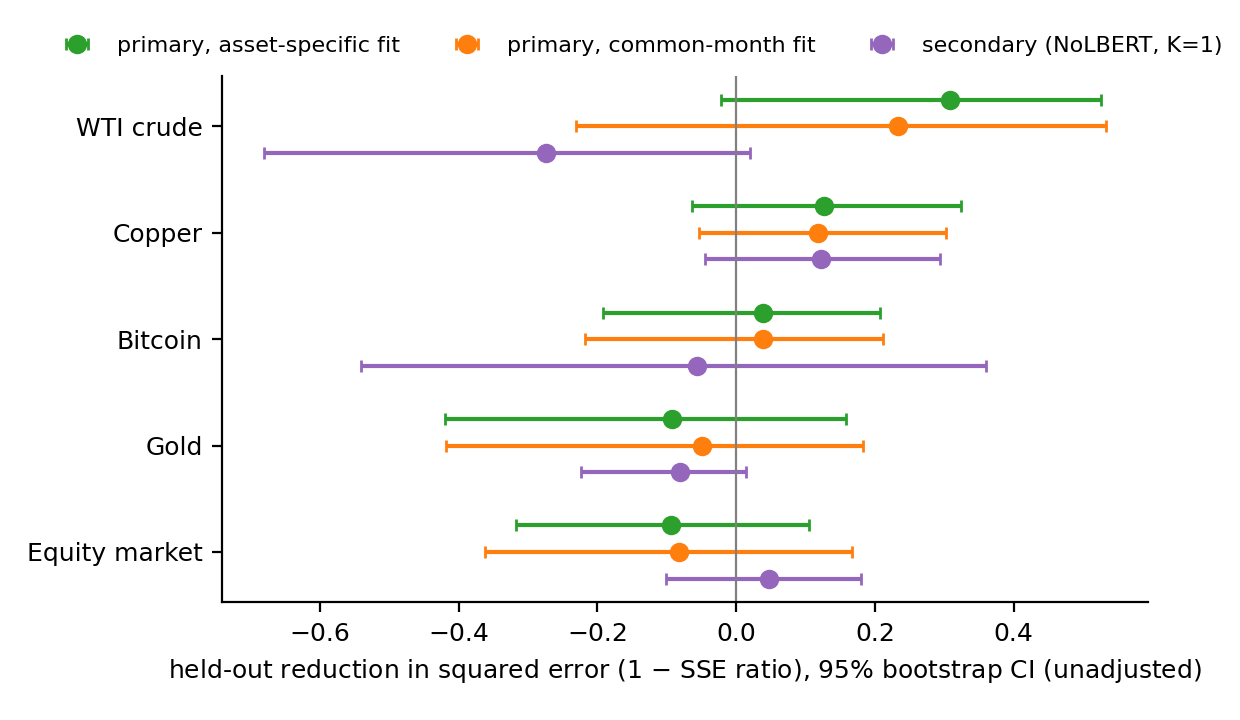
\includegraphics[width=0.78\textwidth]{figures/fig_heldout_gain.png}
\caption{Held-out reduction in squared error relative to the equity-market benchmark, 21 test months. Dots are point estimates, bars unadjusted 95\% bootstrap intervals. Only crude oil has a clearly positive point estimate under the primary model, its interval reaches zero, and the secondary model does not reproduce it.}
\label{fig:gain}
\end{figure}

\paragraph{Calibrating the test.} The Clark--West approximation is justified for a small test sample relative to the estimation sample, and here 21 test months sit beside 59 or 28 fit months. We therefore simulated the whole procedure under the null that the factors add nothing, generating returns from the fitted benchmark with wild-bootstrap residuals and holding the observed market and factor values fixed (5{,}000 draws). The analytic test is not badly off: at a nominal 5\% it rejects between 4.2\% and 8.4\% of the time across assets and samples. Referring the statistic to the simulated null instead gives a calibrated $p$-value of 0.017 for crude oil and a Holm-adjusted value of 0.066. A third, post hoc version that uses the gain itself as the statistic puts crude oil's raw $p$-value at 0.006 and the Holm-adjusted value at 0.022 (the gain of 0.31 exceeds the 95th percentile of its null distribution, 0.17); on the common-month sample the same adjusted value is 0.162 (Appendix~\ref{app:calib}, Table~\ref{tab:calib}). The crude-oil result is thus \emph{borderline}: not significant under the pre-specified inference or the calibrated Clark--West statistic, but crossing the conventional line under one post hoc alternative. We do not treat that alternative as confirmation, since it was not specified in advance, the sample is 21 months, and the correction ignores the dependence between assets.

\paragraph{Other assets.} Copper shows a small, similar gain under both models (0.13 for the primary and 0.12 for the secondary; adjusted $p$ of 0.108 and 0.245), the only pattern that repeats across the two specifications. Gold and Bitcoin show no held-out gain ($-0.09$ and 0.04), and the equity market itself is not explained ($-0.09$), as one would expect for factors built from returns relative to the cross-sectional mean. The secondary NoLBERT factor does not reproduce the crude-oil result (gain $-0.27$ for crude, $-0.08$ for gold, $-0.06$ for Bitcoin).

\paragraph{Joint tests, reported separately.} Our original specification listed one joint test per asset: that the factor coefficients are jointly zero, estimated on the 21 test months themselves. After review we classify these as descriptive, because the coefficients are re-estimated in the sample being evaluated, and keep them apart from the held-out comparison above (Table~\ref{tab:joint}). None is significant under HC3, with or without adjustment; the calendar-aware Newey--West version, which links only neighbouring calendar months, gives 0.031 for Bitcoin, which does not survive the adjustment (0.123). The minimum incremental $R^2$ that 21 months could detect with 80\% power is 0.31 to 0.39.

\begin{table}[t]
\centering\small
\begin{tabular}{@{}lccccrc@{}}
\toprule
 & \multicolumn{3}{c}{All available months} & \multicolumn{3}{c}{21 test months, re-estimated} \\
\cmidrule(lr){2-4}\cmidrule(l){5-7}
Asset & $n$ & $\Delta$ adj.\ $R^2$ & Joint $p$ & $n$ & Joint $p$ & Holm $p$ \\
\midrule
WTI crude & 80 & 0.20 & $<0.001$ & 21 & 0.443 & 1.000 \\
Copper & 80 & 0.04 & 0.060 & 21 & 0.719 & 1.000 \\
Bitcoin & 49 & 0.03 & 0.116 & 21 & 0.234 & 0.938 \\
Gold & 80 & 0.01 & 0.176 & 21 & 0.550 & 1.000 \\
\bottomrule
\end{tabular}
\caption{Descriptive fit of the primary model (M2 against the equity-market benchmark M0): increase in adjusted $R^2$ and the joint test that the factor coefficients are zero (HC3). These estimates are not out-of-sample evidence; the held-out comparison is in Table~\ref{tab:heldout}.}
\label{tab:joint}
\end{table}

\begin{figure}[t]
\centering
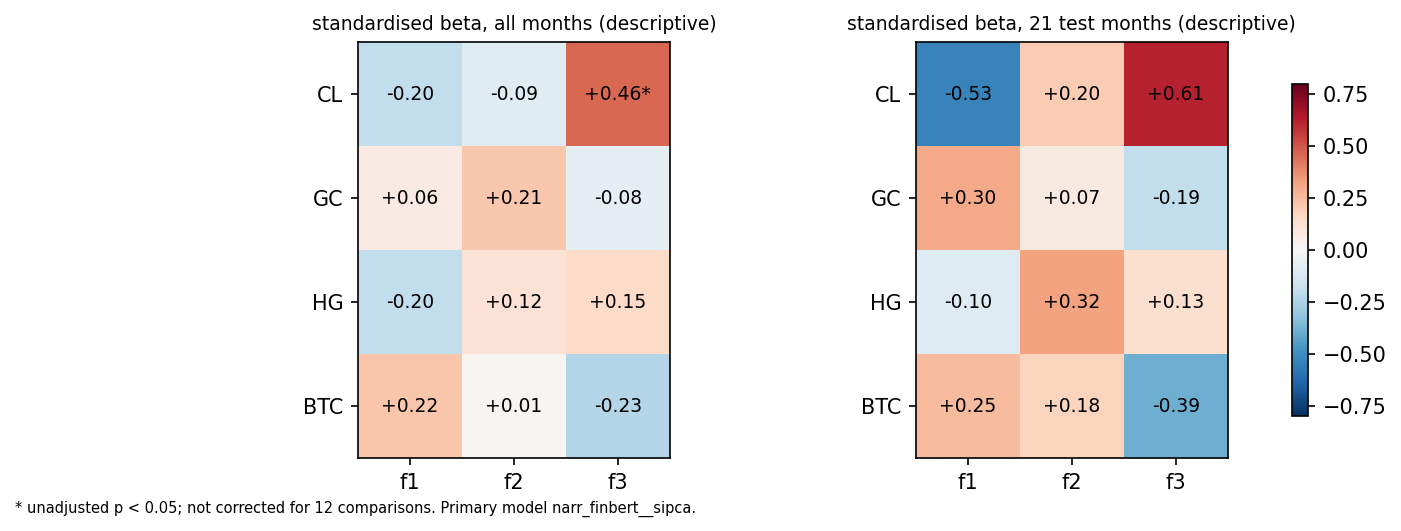
\includegraphics[width=0.82\textwidth]{figures/fig_exposure_heatmap.png}
\caption{Standardised factor exposures of each futures market (primary model, all months and the 21 test months). Both panels are descriptive; asterisks mark unadjusted $p<0.05$ without correction for the twelve comparisons. Crude oil's exposure to the third factor is the largest and keeps its sign in the test months.}
\label{fig:heat}
\end{figure}

\paragraph{Post hoc robustness: shock window, representation and 2024.} Three checks followed the main analysis. Because the 21 test months had already been examined, they are post hoc, not independent confirmation, and the original 5-day FinBERT result stays primary. We fixed them in writing before running them, used only saved specifications, and changed no factor count, penalty, asset or sample.

\emph{The 63-day window.} The pipeline's validation selected a 63-day shock window for monthly rebalancing. Three saved narrative-only specifications use it with $K=3$ factors: FinBERT-20, NoLBERT-20 and LDA-60, so NoLBERT and FinBERT can now be compared at the same $K$ and window. The 63-day feature blocks are not saved, so we re-implemented the project's pipeline and checked it: it reproduces the saved 5-day feature blocks (per-date rank correlation 1.000) and the saved 63-day factor returns (correlation at least 0.998, and 0.993 in the test months), and it uses only news dated at least one day before each formation date. Table~\ref{tab:robust} gives the results. With FinBERT the crude-oil link persists and is larger under the 63-day window: gain 0.25 ([0.04, 0.46]), Holm-adjusted $p=0.018$ across its four assets and 0.054 (analytic) or 0.043 (calibrated) across all twelve tests of the three 63-day specifications. With NoLBERT at the same $K$ and window the link does not appear ($-0.16$, [$-0.50$, 0.23]), and with LDA the gain is small and not significant after adjustment (0.10, [$-0.15$, 0.35]; Holm $p=0.155$). Gains for copper, gold and the equity market are small or negative in all three 63-day specifications, so copper's small original gain does not carry over clearly. The factor most associated with crude oil under FinBERT-63 is again not the one that loads on Energy/Oil (standardised coefficients +0.06 for the Energy/Oil-loaded $f_1$ and $-$0.40 for $f_3$, which loads on Analyst Update, Financials and General News). One result runs the other way: NoLBERT with the 63-day window shows a Bitcoin gain of 0.31 ([0.01, 0.48]), Holm-adjusted 0.050 among four assets and 0.136 among twelve. Its loadings are on analyst-blog, dividend and market-wrap topics, with nothing about crypto-assets, and Bitcoin has only 28 fitting months, so we do not interpret it: one such result in twelve tests is not surprising.

\emph{2024.} Dropping the seven test months with formation on or after 1 December 2023, where the news source changes, and keeping the frozen coefficients, leaves crude oil's gain at 0.33 ([$-0.06$, 0.59]; Holm $p=0.147$ analytic, 0.114 calibrated) against 0.31 with all 21 months. The crude result does not depend on the affected months, although 14 months cannot rule out modest differences.

\emph{Reading.} The link between FinBERT-based factors and crude oil appears under both windows, whereas neither of the two historically more compatible representations reproduces it at comparable strength. That is what one would expect if the result depends on the representation, either because the FinBERT classes capture something the others miss or because the classifier's later information helps. We cannot tell which. We therefore describe the crude-oil result as representation-dependent, suggestive evidence of contemporaneous explanation, and not as evidence of predictive power or of an investable signal.

\begin{table}[t]
\centering\footnotesize
\begin{tabular}{@{}p{0.27\linewidth}p{0.11\linewidth}p{0.17\linewidth}ccccc@{}}
\toprule
 & & \multicolumn{3}{c}{Crude oil} & \multicolumn{3}{c}{Gain, other assets} \\
\cmidrule(lr){3-5}\cmidrule(l){6-8}
Specification & Representation & Gain [95\% CI] & Holm (4) & Holm (12) & Copper & Gold & Bitcoin \\
\midrule
FinBERT-20, 5-day, $K=3$ (original primary) & not point-in-time & 0.31 [$-0.02$, 0.53] & 0.103 & --- & 0.13 & $-0.09$ & 0.04 \\
NoLBERT-20, 5-day, $K=1$ (original secondary) & more compatible & $-0.27$ [$-0.68$, 0.02] & 1.000 & --- & 0.12 & $-0.08$ & $-0.06$ \\
FinBERT-20, 63-day, $K=3$ & not point-in-time & 0.25 [0.04, 0.46] & 0.018 & 0.054 & 0.08 & $-0.03$ & 0.09 \\
NoLBERT-20, 63-day, $K=3$ & more compatible & $-0.16$ [$-0.50$, 0.23] & 1.000 & 1.000 & $-0.07$ & $-0.07$ & 0.31 \\
LDA-60, 63-day, $K=3$ & more compatible & 0.10 [$-0.15$, 0.35] & 0.155 & 0.386 & 0.03 & 0.02 & $-0.14$ \\
\bottomrule
\end{tabular}
\caption{Original (5-day) and post hoc 63-day results side by side, held-out gain over the equity-market benchmark in the 21 test months, same fit months and test months for every specification. Holm (4): across the four assets within a specification (analytic Clark--West); Holm (12): across all twelve asset-model tests of the three 63-day specifications (conservative post hoc family), shown only for them. The 63-day results are post hoc and do not replace the original primary result. ``More compatible'': historically more compatible with the test period, not free of look-ahead.}
\label{tab:robust}
\end{table}

\section{Economic Interpretation}
\label{sec:interp}

It is tempting to read the crude-oil result as oil news explaining oil prices. The factor loadings do not support that reading. In the primary model the factor most associated with crude oil, $f_3$ (standardised coefficient 0.46 over all months, descriptive), loads mostly on Analyst Update ($-$0.53), Stock Movement (+0.43), Earnings ($-$0.35), Markets (+0.32) (Figure~\ref{fig:heat}). The factor that loads on the Energy/Oil class, $f_1$ (together with Currencies (+0.41), Energy | Oil (+0.38), Gold | Metals | Materials ($-$0.36), M\&A | Investments ($-$0.34)), has an insignificant coefficient for crude over all months ($-1.06$, $p=0.12$). The second factor loads on Treasuries | Corporate Debt (+0.63), General News | Opinion ($-$0.43), Gold | Metals | Materials ($-$0.26), Analyst Update (+0.26).

We treat this mismatch as a prompt for caution, not as a finding. The factors are latent, their signs and rotations arbitrary, and what we call a loading is a weight on a stock's return covariance with narrative shocks, not on a topic's weight directly, so the largest loadings alone do not tell us what a factor ``is''. One possibility is that $f_3$ summarises broad market activity, earnings-season and sentiment conditions that also move crude oil. Another is that energy-related news matters through channels the Energy/Oil class does not isolate. A third is chance. We ran no analysis that could tell these apart, and the result that the historically more compatible NoLBERT factor does not reproduce the link makes the first reading no more or less plausible.

The more general point is that explanation can arise from common economic conditions. If attention to earnings and market movement, the factors and crude-oil returns all respond to the same macroeconomic state, the factors carry information about that state without carrying anything specific to oil that a forecaster could exploit.

\section{Comparing the Two Experiments}
\label{sec:compare}

Table~\ref{tab:compare} and Figure~\ref{fig:phase} set the evidence side by side. The experiments differ in universe, frequency, target, inputs and evaluation, so the rows are not comparable performance tests. The table shows what kind of claim each can support.

\begin{table}[t]
\centering\footnotesize
\begin{tabular}{@{}p{0.15\linewidth}p{0.40\linewidth}p{0.38\linewidth}@{}}
\toprule
 & Phase 1: topic-based forecasting & Phase 2: IPCA factors \\
\midrule
Question & Do topic signals forecast returns? & Do equity-derived factors explain same-month futures returns? \\
Targets & Stock deciles (monthly, biweekly, weekly); weekly oil, gold and Bitcoin futures & Monthly crude, copper, gold and Bitcoin futures; the equity market \\
Test sample & 21 / 42 / 81 periods (stocks); 149 weeks (futures) & 21 months \\
Evaluation & Sharpe ratio after costs, bootstrap, deflated Sharpe; weekly out-of-sample $R^2$ against the historical mean & Held-out squared-error gain over the equity market; descriptive fit on all months \\
Evidence type & Forecasting & Contemporaneous explanation \\
Headline & Validation winners fall to Sharpe $-0.17$, 0.40, 0.07 after 10 bp; no weekly forecasting gain & Crude gain 0.31 [$-0.02$, 0.53]; copper 0.13; gold and Bitcoin none \\
After adjustment & Weekly tests: none survives (Holm $p\geq 0.103$). Stocks: deflated Sharpe at most 0.75 & Pre-specified: none survives (Holm $p\geq 0.103$); crude borderline under alternatives \\
Costs & Charged, 0--20 bp per side & Not applicable \\
\bottomrule
\end{tabular}
\caption{The two experiments side by side. They use different data, frequencies, targets and evaluation rules, and should not be read as a horse race.}
\label{tab:compare}
\end{table}

\begin{figure}[t]
\centering
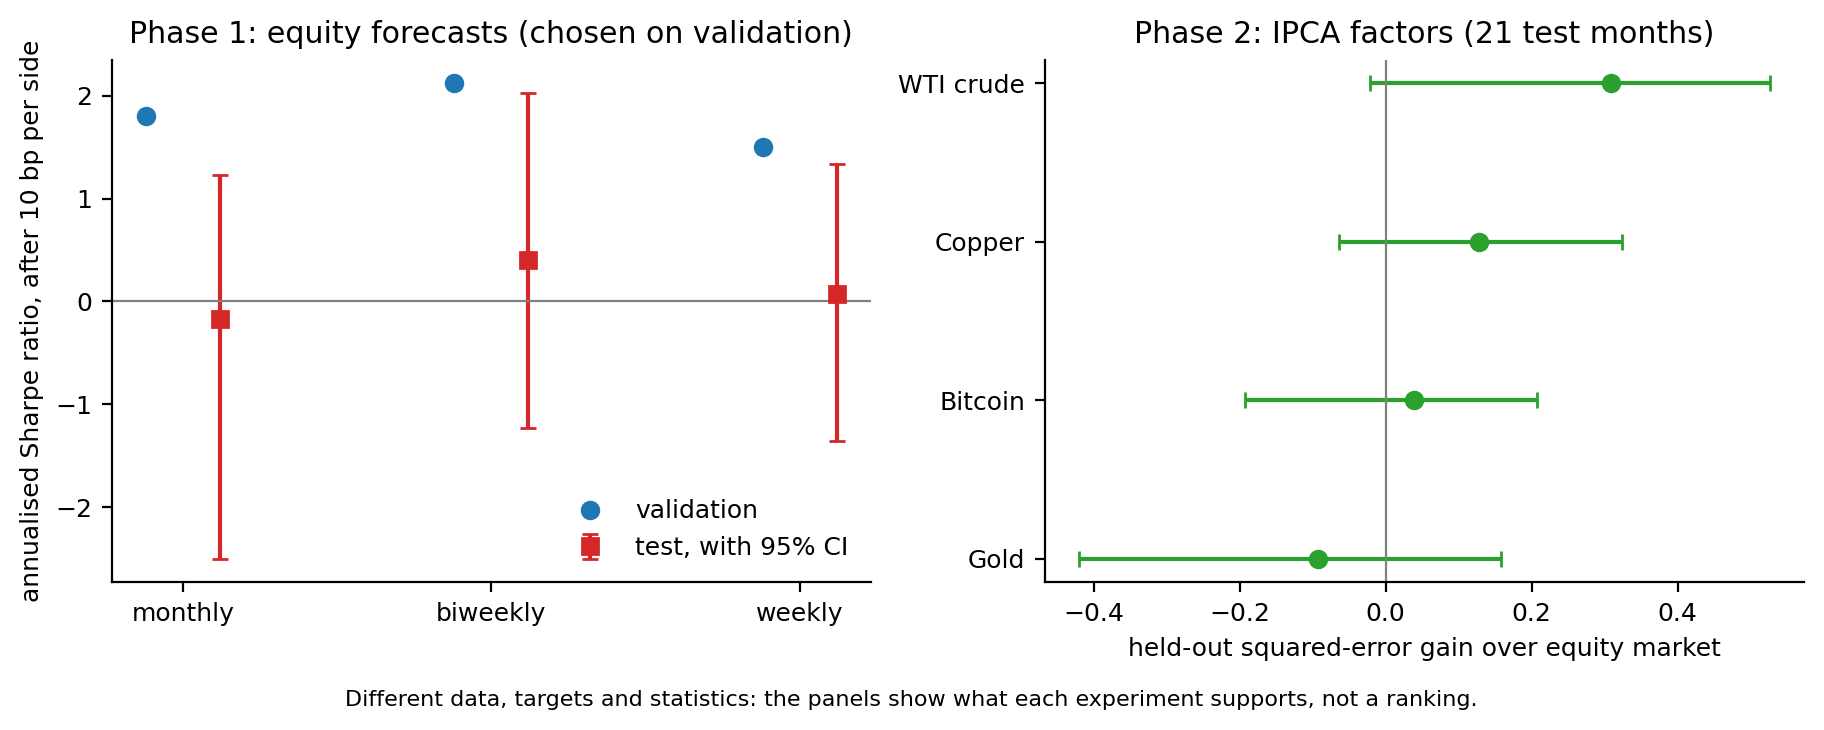
\includegraphics[width=0.95\textwidth]{figures/fig_phase_comparison.png}
\caption{Left: Phase 1, validation Sharpe ratio of the specification chosen on validation and its test Sharpe ratio with a 95\% block-bootstrap interval, after 10 basis points. Right: Phase 2, held-out squared-error gain with unadjusted 95\% intervals. The two panels have different units and answer different questions; what they share is that the apparent strength in sample or validation shrinks, or becomes uncertain, in the held-out period.}
\label{fig:phase}
\end{figure}

\section{Limitations and Implications}
\label{sec:limits}

\paragraph{Sample size and power.} (A fuller audit of data restrictions is in Appendix~\ref{app:audit}.) Twenty-one held-out months is a small sample for a regression with a benchmark and three factors. The smallest incremental $R^2$ we could detect with 80\% power is 0.31 to 0.39, so a gain of 0.31 in squared error is close to the smallest effect the design could reliably detect, and the small positive results for copper and Bitcoin neither confirm nor rule out modest effects. The months are not contiguous, and robust standard errors do not model dependence between neighbouring months.

\paragraph{A short, non-contiguous evaluation sample.} The 21 test months are the December 2021 formation and the June--December formations of 2022--2024, that is the holding months January and July--December. February--June holding months are absent by design, because the daily return file lacks the stocks that would not yet be in the June list; they are not a gap we chose. The results therefore speak only to those holding months: any seasonal difference in commodities or in the factor relationship in the omitted months is unobserved. The bootstrap resamples months as if they were exchangeable, but 17 of the 20 successive pairs of test months are adjacent calendar months, so serial dependence in the errors would make our intervals too narrow, and the robust standard errors do not model it either. We could not validate this without a new analysis, for example a block bootstrap, which we did not run. As a diagnostic on the frozen results, the first-order correlation of the monthly loss differential between adjacent months is 0.30 for crude, $-0.10$ for gold, $-0.34$ for copper and 0.08 for Bitcoin; with 17 pairs each is within about 1.5 standard errors (roughly 0.24) of zero, so the diagnostic neither confirms nor rules out dependence. With 21 months, and 14 once 2024 is dropped, only large effects are detectable, and annualised Sharpe ratios computed from non-contiguous periods are approximate.

\paragraph{Multiple testing.} The equity study ran 375 real specifications, and the cross-asset experiments each ran a family of eight or four primary tests. We corrected within families but not across the whole project, and the robustness checks add further looks.

\paragraph{Point-in-time representations.} The text representations differ in how safe they are from look-ahead. The FinBERT classes are not point-in-time: the classifier was published in December 2022 and fine-tuned on a finance-tweet dataset published in September 2022, whose tweets' own dates are not stated. Our primary factor model uses them, as do two of the three validation-selected equity specifications. NoLBERT was pretrained on text from 1976 to 1995 and is adapted to news with a text-only objective that uses no returns. According to the project documentation, the adaptation drew headline--lead pairs from our corpus up to 1 September 2020, the training end of an earlier pipeline rather than the 31 December 2019 training end used here, so eight months of our validation period (January--August 2020) entered the adaptation; the project accepted this knowingly because it affects validation-period numbers and not the test period. The documented remedy, re-adapting with the earlier cutoff, has not been done, and the 2022--2024 test period is unaffected. Only the NoLBERT-based features are affected by the encoder overlap: the secondary factor model, one of the two oil definitions, and some equity specifications. The representation that shows the crude-oil pattern, in both the 5-day and the 63-day versions, is the one that is not point-in-time, and the two historically more compatible representations do not reproduce it at comparable strength. NoLBERT and LDA are not free of look-ahead either, since the encoder adaptation overlaps the validation period and the vocabulary basis comes from the whole corpus, so ``more compatible'' is a matter of degree. We cannot say whether the difference reflects look-ahead in the classifier or simply better class definitions.

\paragraph{Shock window and sample.} The \texttt{\_s63} variants use a 63-day shock window that validation chose for monthly rebalancing. Our monthly analyses, including the saved monthly stock forecasts, use the default five-day window and so are not the configuration the pipeline's validation preferred at that frequency; we make no claim that they reproduce it. We therefore ran the factor analysis on the saved 63-day factors as a post hoc check (Section~\ref{sec:results}); the monthly stock forecasts of Phase 1 were not rebuilt with 63-day features. The stock panel omits February--June holding months from 2017 by design: from 2017 the daily return file holds only the stocks of each year's June list, so features observed before the list changes would be observed for a sample selected on the future, and those formation days are left out. This avoids a look-ahead but means the test sample is 21 of 36 months. The 2024 news is thinner, partly headline-only and drawn from a different source than earlier years; this is a potential distribution shift in the last part of the test window that could move out-of-sample results in either direction, and we did not test for it. About 1.1\% of monthly stock observations belong only to the following June's universe, a small look-ahead we did not quantify. Futures data begin in 2015 (December 2017 for Bitcoin), and Bitcoin has no crypto-specific narrative.

\paragraph{Interpretation.} Even the strongest result is consistent with a common-cause account in which news attention, the factors and crude-oil returns respond to the same macroeconomic conditions. An explanatory gain cannot distinguish a common cause from information that matters for oil specifically, and it says nothing about tradability.

\section{Conclusion}
\label{sec:conclusion}

Our results suggest that financial-news narratives may contain information relevant to cross-asset price movements, particularly crude oil. The FinBERT-based factors reduced held-out squared error by approximately 31\% relative to the equity-market benchmark. However, this improvement did not survive the pre-specified multiple-testing adjustment (Holm-adjusted $p=0.103$; 0.066 with a simulation-calibrated reference distribution, and 0.022 for a post hoc version that uses the gain itself), so its statistical significance is sensitive to the inference method. The interval for the gain reaches zero, the result weakens on common months, the factor responsible does not look like an energy factor, and the historically more compatible representations do not reproduce it: a post hoc check with the pipeline's 63-day window and the same number of factors shows the link again with FinBERT (gain 0.25) but not with NoLBERT ($-0.16$), and only weakly with LDA (0.10). In stocks, our evidence cannot tell signal from luck: validation winners do not hold up in the test period, costs remove most of what is left, and, at the monthly frequency, a shuffled placebo does about as well as the best real specification. For commodities and Bitcoin, weekly topic-attention shocks move with crude-oil returns but forecast nothing. Gold shows no relationship in either experiment, and Bitcoin none in the original analyses; the one post hoc Bitcoin gain, with NoLBERT at 63 days, does not survive the twelve-test adjustment and has no crypto-related content. Overall, we find suggestive evidence of common information across equity news and commodity markets, and describe the crude-oil result as representation-dependent explanation, not predictive power. The evidence is insufficient to establish a robust forecasting or trading signal.

We think the negative findings are informative. They separate three things that are easy to conflate: a text representation that yields coherent and interpretable topics, factors whose exposures explain some return variation in some markets, and signals that forecast returns well enough to trade. The evidence supports the first, offers suggestive but unconfirmed support for the second, and does not support the third. The natural next steps are a larger held-out sample, a prespecified test of the crude-oil relationship on data we have not used, re-adapting the encoder with the 2019 cutoff and rebuilding the monthly stock forecasts with 63-day features, and a clearer account of what the third factor captures.

\paragraph{Why not trade on it?} If the factors help explain crude-oil returns, why can an investor not use them? Because the relationship we measure is contemporaneous: the factors are estimated from same-month stock returns, so they are not known before the return they are compared with. And the primary factors rest on a representation that is not point-in-time, so even the historical relationship is not a clean statement about what could have been known. A forecasting or trading claim would need both conditions to be different, and our forecasting tests, which use only news dated before the return window, find nothing.

\section*{References}
\begin{description}\setlength{\itemsep}{0pt}
\item Bailey, D.~H., and M.~L\'opez de Prado (2014). The deflated Sharpe ratio: correcting for selection bias, backtest overfitting, and non-normality. \emph{Journal of Portfolio Management} 40(5), 94--107.
\item Bybee, L., B.~Kelly, and Y.~Su (2023). Narrative asset pricing: interpretable systematic risk factors from news text. \emph{Review of Financial Studies} 36(12), 4759--4787.
\item Clark, T.~E., and K.~D.~West (2007). Approximately normal tests for equal predictive accuracy in nested models. \emph{Journal of Econometrics} 138(1), 291--311.
\item Dong, Z., X.~Fan, and Z.~Peng (2024). FNSPID: a comprehensive financial news dataset in time series. arXiv:2402.06698.
\item FinMultiTime (n.d.). Hugging Face dataset repository \url{Wenyan0110/Multimodal-Dataset-Image_Text_Table_TimeSeries-for-Financial-Time-Series-Forecasting}, file \texttt{text/sp500\_news.zip}. MIT licence.
\item French, K.~R. (n.d.). Kenneth R.~French Data Library, \url{https://mba.tuck.dartmouth.edu/pages/faculty/ken.french/data_library.html}.
\item Holm, S. (1979). A simple sequentially rejective multiple test procedure. \emph{Scandinavian Journal of Statistics} 6(2), 65--70.
\item Kakhbod, A., and P.~Li (2025). NoLBERT: a no lookahead(back) foundational language model. arXiv:2509.01110.
\item Kelly, B.~T., S.~Pruitt, and Y.~Su (2019). Characteristics are covariances: a unified model of risk and return. \emph{Journal of Financial Economics} 134(3), 501--524.
\item nickmuchi (2022). Hugging Face model repository \url{nickmuchi/finbert-tone-finetuned-finance-topic-classification}, created 30 December 2022; fine-tuned on the dataset \url{zeroshot/twitter-financial-news-topic} (repository created 7 September 2022; the tweets' collection dates are not stated).
\item MacKinnon, J.~G., and H.~White (1985). Some heteroskedasticity-consistent covariance matrix estimators with improved finite sample properties. \emph{Journal of Econometrics} 29(3), 305--325.
\item Newey, W.~K., and K.~D.~West (1987). A simple, positive semi-definite, heteroskedasticity and autocorrelation consistent covariance matrix. \emph{Econometrica} 55(3), 703--708.
\end{description}

\appendix
\section{Data-Leakage and Reproducibility Audit}
\label{app:audit}

\small
\begin{longtable}{@{}p{0.2\linewidth}p{0.2\linewidth}p{0.55\linewidth}@{}}
\toprule
Item & Status & Detail \\
\midrule
\endhead
Factor estimation schedule & Documented; consistent with saved files & Grid fitted on training months, chosen on validation error, refitted once on training and validation, applied unchanged to test months; train and validation factor months flagged in-sample, test months out-of-sample; the project's own reproduction of the saved test forecasts agrees to $10^{-9}$ (29 of 50 specifications reproduced independently). \\ \midrule
Characteristic scaling and windows & Verified & Cross-sectional ranks within each date; exposure windows end at the formation date (rebuilt from daily attention and returns; rank correlation 0.92, falling to 0.72 and 0.41 when shifted forward by 21 and 63 days). \\ \midrule
Topic models and vocabulary & Documented; metadata verified & Clustering fitted on articles through 2019-12-31 only; the 10{,}000-term vocabulary basis comes from the whole corpus (project documentation). \\ \midrule
NoLBERT representation & Historically more compatible; validation overlap documented & Pretrained on 1976--1995 text; adapted on news with a headline--lead matching objective that uses no returns, on pairs drawn up to 1 September 2020 (project documentation), so eight validation months overlap; test period unaffected. \\ \midrule
FinBERT representation & Issue: not point-in-time & Classifier published December 2022 and fine-tuned on a finance-tweet dataset published September 2022 (repository creation dates; tweet dates not stated). The primary factor model and two of three validation-selected equity specifications use it. \\ \midrule
Shock window & Issue, partly addressed post hoc & The validation-chosen window for monthly rebalancing is 63 days; the main analyses use the default five days. The saved 63-day factors were analysed post hoc; the monthly stock forecasts were not rebuilt. \\ \midrule
Feature reproducibility & Verified & A re-implementation of the project's pipeline reproduces the saved 5-day feature blocks (rank correlation 1.000) and the saved 63-day factor returns (correlation at least 0.998; test months at least 0.993). \\ \midrule
News cutoff & Verified in code & Exposures use shock days up to the day before the formation date (lag of one day), because article dates carry no time of day. \\ \midrule
Feb--Jun holding months & Documented & From 2017 the daily return file holds only each year's June-list stocks, so formation days before the list changes are left out to avoid features observed for a sample selected on the future. \\ \midrule
Calendar alignment & Verified & Holding window is the following calendar month; matches compounded stock returns for all 104 months; windows of consecutive months do not overlap. \\ \midrule
Stock universe & Verified; one issue & 98.7\% of monthly rows belong to the list formed at the latest June; about 1.1\% belong only to the next June's list. \\ \midrule
News sources, 2024 & Documented & FNSPID and FinMultiTime; 1{,}255{,}289 articles; one dump day removed; 22 articles in January 2024; about 4{,}500 articles of 2024 have only headlines. \\ \midrule
Intraday timing of news & Cannot be verified & Articles carry dates, not times; the forecasting design skips the last trading day of the week. \\ \midrule
\bottomrule
\end{longtable}
\normalsize

\section{Inference for the Held-Out Tests}
\label{app:calib}

\begin{table}[h]
\centering\small
\begin{tabular}{@{}lcccccc@{}}
\toprule
 & \multicolumn{2}{c}{Analytic Clark--West} & \multicolumn{2}{c}{Calibrated Clark--West} & \multicolumn{2}{c}{Gain as statistic (post hoc)} \\
\cmidrule(lr){2-3}\cmidrule(lr){4-5}\cmidrule(l){6-7}
Asset & $p$ & Holm & $p$ & Holm & $p$ & Holm \\
\midrule
WTI crude & 0.026 & 0.103 & 0.017 & 0.066 & 0.006 & 0.022 \\
Copper & 0.036 & 0.108 & 0.045 & 0.134 & 0.044 & 0.133 \\
Bitcoin & 0.095 & 0.189 & 0.130 & 0.259 & 0.168 & 0.336 \\
Gold & 0.509 & 0.509 & 0.558 & 0.558 & 0.656 & 0.656 \\
\bottomrule
\end{tabular}
\caption{Three ways of computing inference for the primary held-out comparison (asset-specific fit sample; Holm over the four assets). Analytic: pre-specified, referred to a normal-theory distribution. Calibrated: the same statistic referred to its distribution under the null, simulated with 5{,}000 wild-bootstrap draws that hold the observed market and factors fixed. The gain-based version was added after review and is post hoc.}
\label{tab:calib}
\end{table}

\end{document}
